\documentclass[a4paper, twocolumn, 11pt, twoside]{article}

\usepackage[portuguese]{babel}
\usepackage{linguamatica}
\usepackage{amsmath}
\usepackage{microtype}
\usepackage{makecell}
\usepackage{array}
\usepackage{icomma}

\bibliographystyle{sp_por}

\submitted{}
\accepted{}

\title{Avaliação de Modelos de Linguagem de Grande Escala para Simplificação Textual em Português Brasileiro com Diferentes Estratégias de Prompting e Fine-Tuning}

\titleEN{Evaluation of Large Language Models for Text Simplification in Brazilian Portuguese with Different Prompting and Fine-Tuning Strategies}

\author{
  João Pedro Hallack Sansão
  \href{https://orcid.org/0009-0002-1697-4033}{0009-0002-1697-4033}
  \instituto{Departamento de Tecnologia --- DTECH \\ Universidade Federal de São João del-Rei (UFSJ)}
  \email{joao@ufsj.edu.br}
}


\begin{document}

\maketitle

\begin{resumo}
A simplificação textual é uma tarefa fundamental do Processamento de
Linguagem Natural que visa reduzir a complexidade linguística de textos,
preservando seu significado original. Este trabalho avalia cinco LLMs
(GPT-4o mini, GPT-4o, Claude Sonnet 4.6, Llama 4 Scout e Qwen 2.5 7B)
na tarefa de simplificação textual para o português brasileiro,
utilizando o dataset PorSimplesSent. Testamos três estratégias
de prompting (zero-shot, few-shot, chain-of-thought) e fine-tuning de
três variações do PTT5-small (60M) com LoRA rank 8, rank 32 e
fine-tuning completo, além do Qwen 2.5 0.5B com QLoRA.
As métricas incluem ROUGE, BERTScore, SARI, e índices de legibilidade
Flesch e Gunning-Fog adaptados para o português. Os resultados mostram
que Claude Sonnet 4.6 (few-shot, SARI=42,6) e Qwen 2.5 7B (few-shot, SARI=41,7) obtêm os melhores escores de
similaridade (ROUGE-1 $\geq$ 0,66), enquanto o Llama 4 Scout alcança os maiores ganhos de
legibilidade (Flesch $\Delta = +13,2$, Fog $\Delta = -4,0$).
O fine-tuning do PTT5-small supera todos os
resultados de prompting em similaridade (ROUGE-1 até 0,74, SARI até
55,5). Isso mostra que o treinamento em domínio específico compensa a
diferença de escala. Uma avaliação complementar
LLM-as-judge com dois modelos juízes (Gemini 3.1 Flash Lite e GPT-4o
mini) confirma a fluência e adequação
das simplificações, mas revela limitações qualitativas nos
modelos fine-tunados e baixa concordância entre juízes automáticos para modelos
de prompting.
\end{resumo}

\palavraschave{simplificação textual; LLMs; prompting; fine-tuning; português brasileiro}

\begin{abstract}
Text simplification is a fundamental Natural Language Processing task that
aims to reduce the linguistic complexity of texts while preserving their
original meaning. This work evaluates five LLMs
(GPT-4o mini, GPT-4o,
Claude Sonnet 4.6, Llama 4 Scout, and Qwen 2.5 7B)
on text simplification
for Brazilian Portuguese using the PorSimplesSent dataset. We test three
prompting strategies (zero-shot, few-shot, chain-of-thought) and fine-tune
three PTT5-small (60M) variants with LoRA rank 8, rank 32, and full
fine-tuning, plus Qwen 2.5 0.5B with QLoRA.
Metrics include ROUGE, BERTScore, SARI, and Flesch and Gunning-Fog
readability indices adapted for Portuguese. Results show that Claude Sonnet 4.6 (few-shot, SARI 42.6) and Qwen 2.5 7B (few-shot, SARI 41.7) achieve the best similarity scores (ROUGE-1 $\ge$ 0.66), while Llama 4 Scout obtains the
largest readability gains (Flesch $\Delta = +13.2$, Fog $\Delta = -4.0$).
Fine-tuning the PTT5-small (60M) surpasses all prompting results in similarity
(ROUGE-1 up to 0.74, SARI up to 55.5), demonstrating that domain-specific
training compensates for the scale difference.
A complementary LLM-as-judge evaluation with two judge models
(Gemini 3.1 Flash Lite and GPT-4o mini)
confirms the fluency and adequacy of the simplifications but reveals
qualitative limitations in fine-tuned models and low inter-judge
agreement for prompting-based models.
\end{abstract}

\keywords{text simplification; LLMs; prompting; fine-tuning; Brazilian Portuguese}

\section{Introdução}

A simplificação textual é uma tarefa do Processamento de Linguagem Natural
(PLN) que consiste em reescrever um texto original de modo a reduzir sua
complexidade lexical e sintática, tornando-o mais acessível sem perder o
significado \citep{caseli2009}. Esta tarefa beneficia
públicos com baixa escolaridade, afasias, déficit de atenção e aprendizes
de segunda língua \citep{aluisio2008}.

Tradicionalmente, sistemas de simplificação textual eram construídos com
abordagens baseadas em regras ou em fine-tuning de modelos neurais
\citep{nisioi2017}. No entanto, com o surgimento dos Modelos de Linguagem
de Grande Escala (LLMs) e técnicas de prompting como few-shot
\citep{brown2020} e chain-of-thought \citep{wei2022}, torna-se possível
realizar simplificação textual sem necessidade de treinar o modelo.

Embora existam diversos estudos avaliando LLMs para simplificação textual
em inglês \citep{feng2023,kew2023bless,agrawal2023controlling,farajidizaji2024},
há uma carência de trabalhos focados no português
brasileiro. Este artigo aborda essa lacuna ao avaliar cinco LLMs
na tarefa de simplificação textual do português, utilizando
três estratégias de prompting e fine-tuning de três variações do
PTT5-small e do Qwen 2.5 0.5B. As métricas empregadas incluem
tanto medidas de similaridade textual quanto índices de
legibilidade, além de uma avaliação complementar LLM-as-judge.

As contribuições deste trabalho são: (i) evidência de que o
fine-tuning de modelo pequeno (PTT5-small, 60M) supera o prompting de
modelos grandes (7B--17B) em similaridade textual (ROUGE-1 até 0,74,
SARI até 55,5), mas com comportamento conservador que limita os ganhos
de legibilidade; (ii) demonstração de que a avaliação LLM-as-judge
apresenta baixa concordância entre juízes ($\alpha = 0,181$ em média),
questionando sua confiabilidade como métrica única para simplificação
textual; e (iii) disponibilização de código, amostra de avaliação e
adaptação dos índices de legibilidade Flesch e Gunning-Fog ao
português com contagem silábica baseada em grupos vocálicos\footnote{%
  Repositório: \url{https://github.com/jsansao/llm-text-simplification-ptbr}
  (GPLv3). Dados originais (PorSimplesSent): CC BY 4.0.}. O restante deste
artigo está organizado como segue: a Seção~2 apresenta os trabalhos
relacionados; a Seção~3 descreve a metodologia, incluindo dataset,
modelos, estratégias de prompting e fine-tuning; a Seção~4 reporta os
resultados experimentais; a Seção~5 discute os resultados; e a
Seção~6 conclui o artigo.

\section{Trabalhos Relacionados}

\subsection{O Dataset PorSimplesSent}

O PorSimplesSent é um dataset de simplificação textual para o português
brasileiro, desenvolvido por \citet{caseli2009}. O corpus contém pares de
frases original--simplificada extraídos de textos jornalísticos, com
simplificações produzidas manualmente por especialistas. A versão utilizada
neste trabalho (pss2) contém 2.370 pares alinhados por comprimento de
sentença, nos quais o texto original foi efetivamente simplificado
(campo \texttt{changed} igual a \texttt{S}).

\subsection{Simplificação Textual com Modelos de Linguagem de Grande Escala}

Com o advento dos LLMs, diversos estudos avaliaram seu potencial para
simplificação textual. \citet{feng2023} analisaram a capacidade
zero-shot e few-shot do ChatGPT e GPT-3.5 em benchmarks de
simplificação de sentenças. Os resultados indicam que LLMs superam
métodos supervisionados anteriores e alcançam qualidade
comparável a anotadores humanos.

\citet{kew2023bless} propuseram o BLESS, um benchmark abrangente que
avaliou 44 LLMs (diferentes tamanhos, arquiteturas e níveis de
acesso) em três domínios (Wikipedia, notícias e textos
médicos). Seus resultados indicam que os melhores LLMs, mesmo sem
treinamento específico em simplificação, competem com sistemas
state-of-the-art treinados em dados paralelos.
\citet{agrawal2023controlling} investigaram o controle do nível de
simplificação em modelos T5 (acessíveis e abertos) para públicos
específicos, propondo a predição de operações de
edição (adição, retenção, deleção) por instância, com resultados
superiores a abordagens baseadas em prompting na época.
\citet{farajidizaji2024} exploraram o uso de zero-shot LLMs para
atingir níveis-alvo de legibilidade, em tarefa de modificação
controlada de textos.

Para o português brasileiro, \citet{scalercio2025evaluating} avaliaram o
desempenho de 26 LLMs para simplificação textual com análise linguística
abrangente, e \citet{scalercio2026legalsim} propuseram o LegalSim-PT,
um dataset para simplificação de documentos jurídicos.
Diferentemente de \citet{scalercio2025evaluating}, que adotaram um único
prompt zero-shot para todos os LLMs, e de \citet{agrawal2023controlling},
que focaram exclusivamente em fine-tuning supervisionado de T5, este
trabalho combina, no mesmo dataset e com as mesmas 200 amostras de
avaliação, três estratégias de prompting (zero-shot, few-shot e
chain-of-thought) em cinco LLMs e fine-tuning de dois modelos, permitindo
comparação direta e controlada entre paradigmas.

\subsection{Métricas de Avaliação}

A avaliação de simplificação textual requer métricas que capturem tanto a
similaridade com a referência humana quanto a melhoria efetiva na
legibilidade \citep{xu2016}.

O ROUGE \citep{lin2004} mede a sobreposição de n-grams entre o texto gerado
e a referência, sendo amplamente utilizado em sumarização e simplificação.
Empregamos as variantes ROUGE-1 (unigramas), ROUGE-2 (bigramas) e ROUGE-L
(maior subsequência comum), reportando a média F1. O BERTScore
\citep{zhang2020} utiliza embeddings contextuais do BERT
(\texttt{bert-base-multilingual-cased}) para calcular
similaridade semântica entre predição e referência, com métricas de
precisão, recall e F1. O SARI \citep{xu2016} foi especificamente
desenvolvido para simplificação textual, comparando o texto gerado com o
original e a referência para medir adições, retenções e deleções de
n-grams; reportamos a média das três operações (implementação da
biblioteca \texttt{evaluate} do HuggingFace).

Além das métricas de similaridade predição--referência, reportamos
também R1$_{OP}$ e BS$_{OP}$ (ROUGE-1 e BERTScore entre o texto
original e a predição). Essas métricas medem o quanto o modelo se
afasta do texto original: valores próximos de 1,0 indicam
simplificações conservadoras (mudanças mínimas), enquanto valores
baixos sugerem simplificações mais agressivas.

Para legibilidade, o índice Flesch Reading Ease \citep{flesch1948}
estima a facilidade de leitura com base na extensão das sentenças e no
número de sílabas por palavra. O Gunning-Fog \citep{gunning1952}
estima o nível de escolaridade necessário para compreender o texto.
Ambos foram adaptados para o português com contagem de sílabas
baseada em grupos vocálicos.

\section{Metodologia}

\subsection{Dataset e Pré-processamento}

Utilizamos o dataset PorSimplesSent versão pss2
(\texttt{pss2\_align\_length\_ori\_nat.tsv}), contendo 2.370 pares de
frases original--simplificada. As frases originais têm média de 21,8
tokens, e as simplificadas, 17,6 tokens. Para este experimento,
selecionamos uma amostra estratificada de 200 pares, dividindo o
dataset em tercis de tamanho (número de tokens) e sorteando
proporcionalmente dentro de cada estrato (67/67/66 amostras, seed=42).
A amostra preserva a distribuição
de comprimentos do dataset original: o primeiro tercil contém frases
de até 15 tokens (média 11,6), o segundo de 16 a 24 tokens (média
19,3), e o terceiro acima de 24 tokens (média 34,1). Dessa forma,
a amostra de 200 pares reflete a diversidade de tamanhos do
PorSimplesSent, evitando que frases muito curtas ou muito longas
sejam super-representadas. O tamanho da amostra foi limitado pelo
custo de APIs: cada modelo de prompting requer 3 a 4 chamadas por
amostra, e cada execução LLM-as-judge consome
14--20 chamadas por amostra (9 modelos $\times$ 3 execuções).
Ao todo, são milhares de chamadas de API além dos limites gratuitos
das plataformas. Com n=200, o teste bootstrap pareado (10.000
iterações) tem poder estatístico de 0,80 para detectar diferenças
de $\Delta$R1 $\geq 0,03$ ($\alpha = 0,05$, duas caudas),
suficiente para as comparações realizadas neste trabalho
\citep{cohen1988}.

Identificamos um par (\#16) no qual original e referência tratam de
tópicos distintos (vacinação vs.\ servidora pública), provavelmente um
erro de alinhamento. A amostra foi mantida na análise por representar
cenários reais de ruído em dados de simplificação textual. Durante a
inspeção manual da amostra estratificada, este foi o único par
identificado com esse problema.

\subsection{Modelos Avaliados}

Selecionamos cinco LLMs que representam diferentes categorias:

\begin{itemize}
    \item \textbf{GPT-4o mini} \citep{openai2024gpt4o}: modelo
        proprietário da OpenAI, 8B parâmetros (estimado), 128K tokens
        de contexto.
    \item \textbf{GPT-4o} \citep{openai2024gpt4o}: versão completa do
        modelo da OpenAI, de porte estimado superior (não divulgado).
    \item \textbf{Claude Sonnet 4.6} \citep{anthropic2026claude}: modelo
        proprietário da Anthropic.
    \item \textbf{Llama 4 Scout} \citep{meta2025llama4}: modelo aberto da
        Meta, $\approx$17B parâmetros.
    \item \textbf{Qwen 2.5 7B} \citep{bai2023qwen}: modelo aberto da
        Alibaba, 7B parâmetros.
\end{itemize}

Acessamos todos os modelos via OpenRouter API\footnote{IDs dos modelos: \texttt{openai/gpt-4o-mini}, \texttt{openai/gpt-4o-2024-11-20}, \texttt{anthropic/claude-sonnet-4.6}, \texttt{meta-llama/llama-4-scout-17b-16e-instruct}, \texttt{qwen/qwen-2.5-7b-instruct} (acesso em junho/2026).}.
Os parâmetros de geração foram temperatura 0,0 e limite de 512 tokens de
saída (768 para chain-of-thought). Temperatura 0,0 foi adotada para
garantir reprodutibilidade e comparação justa entre modelos, conforme
prática comum em avaliação de LLMs \citep{zhao2021calibrate}. Todos os modelos foram
avaliados nas estratégias zero-shot e few-shot (k=3); Qwen 2.5 7B,
Llama 4 Scout, GPT-4o mini e GPT-4o foram adicionalmente avaliados com
chain-of-thought. Claude Sonnet 4.6 não foi incluído no experimento
CoT porque o padrão de queda de similaridade já se confirmou
consistentemente nos três modelos de alto desempenho adicionais,
tornando o custo extra de 200 chamadas de API desnecessário para a
análise.

\subsection{Estratégias de Prompting}

Testamos três estratégias de prompting. O zero-shot consiste em
instruir o modelo diretamente sem exemplos. O few-shot
\citep{brown2020} fornece três pares original--simplificada extraídos
do próprio PorSimplesSent como exemplos do comportamento desejado. O
chain-of-thought \citep{wei2022} instrui o modelo a raciocinar passo a
passo antes de produzir a resposta final. O objetivo é verificar
se o raciocínio explícito beneficia a tarefa de simplificação. Os
templates específicos foram:

\begin{enumerate}
    \item \textbf{Zero-shot}: ``Simplifique a frase abaixo em português
        brasileiro. Frase: \{texto\} Simplificação:''
    \item \textbf{Few-shot} (k=3): o prompt acima precedido por três
        pares original--simplificada amostrados aleatoriamente do
        dataset com seed fixa (seed=42) para cada amostra de teste.
        O valor k=3 foi adotado por ser padrão na literatura
        de simplificação textual \citep{brown2020} e por oferecer
        equilíbrio entre fornecer exemplos suficientes e não
        saturar o contexto; uma análise de robustez (Seção~5.4)
        mostra que os resultados são estáveis para
        k entre 1 e 7.
    \item \textbf{Chain-of-thought}: ``Simplifique a frase abaixo. Pense
        passo a passo: identifique palavras difíceis, substitua por
        sinônimos simples, reescreva em ordem direta. Depois do
        raciocínio, escreva a simplificação final em uma nova linha
        começando com 'Simplificação final:'.''
\end{enumerate}

A extração da resposta do modelo foi feita por um parser que identifica
marcadores específicos (``Simplificação final:'') ou, na ausência
destes, seleciona a última linha que não contém marcadores de
raciocínio.

\subsection{Métricas de Legibilidade}

Implementamos um módulo específico de legibilidade para o português. A
contagem de sílabas é feita por um algoritmo baseado em grupos
vocálicos: cada sequência de vogais consecutivas conta como uma
sílaba \citep{aluisio2008}. O índice Flesch adaptado utiliza a fórmula original com a
contagem de sílabas em português:

\begin{equation}
    \text{FRE} = 206,835 - 1,015 \times \frac{P}{F} - 84,6 \times \frac{S}{P}
\end{equation}

onde $P$ é o número de palavras, $F$ o número de frases, e $S$ o
número de sílabas. O Gunning-Fog é calculado como:

\begin{equation}
    \text{Fog} = 0,4 \times \left(\frac{P}{F} + 100 \times \frac{C}{P}\right)
\end{equation}

onde $C$ é o número de palavras complexas ($\geq$ 3 sílabas).
Para cada par original--simplificado, calculamos o delta (melhoria) como
a diferença entre o escore da simplificação e o do original.

\subsection{Experimentos com Fine-Tuning}

Para investigar o potencial do fine-tuning em hardware local limitado,
selecionamos dois modelos abertos e de pequeno porte que cabem em GPUs
com 4~GB de VRAM:

\begin{itemize}
    \item \textbf{PTT5-small} \citep{carmo2020ptt5}: encoder-decoder T5
        de 60 milhões de parâmetros, pré-treinado em português
        brasileiro (BrWac). Fine-tuning com LoRA (rank=8 e rank=32)
        e fine-tuning completo.
    \item \textbf{Qwen 2.5 0.5B} \citep{bai2023qwen}: decoder-only de 0,5
        bilhão de parâmetros, fine-tuning com QLoRA (4-bit NF4,
        rank=16).
\end{itemize}

Realizamos o fine-tuning base nos 1.953 pares de treino (82\% do
PorSimplesSent após remoção do hold-out estratificado por tercil de tamanho de 200 amostras),
com 217 pares reservados para validação. O treinamento
utilizou otimizador AdamW, schedule linear,
learning rate de $2\times10^{-4}$, 10 épocas para o PTT5-small
com LoRA (rank=8, $\alpha=16$, aplicado a {\tt q, k, v, o})
e 5 para o Qwen 2.5 0.5B (QLoRA 4-bit NF4, rank=16, $\alpha=32$,
aplicado a todas as projeções lineares), com batch efetivo de 16
amostras e warmup de 100 iterações (PTT5) e 50 (Qwen).
O PTT5-small (LoRA rank=8) treinou por aproximadamente 3,5
minutos, e o Qwen 2.5 0.5B por 18 minutos em uma NVIDIA GeForce RTX 3050 (4~GB).
Após o treino, cada modelo gerou predições para as mesmas 200 amostras
utilizadas nos experimentos de prompting. Cada configuração foi treinada
uma única vez, sem variação de semente aleatória. Ressaltamos que a
comparação entre fine-tuning e prompting confunde escala do modelo e
paradigma de treinamento: modelos de prompting têm 7B--17B parâmetros
e zero amostras de treino, enquanto os fine-tunados têm 60M--0,5B
parâmetros e 1.953 amostras de treino. Modelos maiores fine-tunados
provavelmente superariam ambos os cenários, mas estavam além do
escopo computacional deste trabalho.

Para investigar se o comportamento conservador do PTT5-small se devia a
underfitting ou à capacidade limitada do adaptador LoRA de baixo posto,
realizamos dois experimentos adicionais: (i) LoRA com rank=32
($\alpha=64$, 2,4 milhões de parâmetros treináveis, 10 épocas, lr=$2\times10^{-4}$)
e (ii) fine-tuning completo (60M parâmetros, 20 épocas,
lr=$5\times10^{-5}$). O treinamento com rank=32 durou aproximadamente
3,5 minutos e o fine-tuning completo, 12 minutos. Todos mantiveram os
mesmos dados e batch efetivo.

\subsection{Avaliação LLM-as-Judge}

Para complementar as métricas automáticas, realizamos uma avaliação
utilizando um modelo de linguagem como juiz (LLM-as-judge).
Neste método, apresentamos a um LLM o texto original, a
referência humana e a saída de um modelo, solicitando avaliações
numéricas nas três dimensões propostas: simplicidade,
fluência e adequação (Likert 1--5). O prompt completo foi:

\begin{quote}\small\em
Você é um avaliador de simplificação textual em português brasileiro.

Você receberá: ORIGINAL (o texto original complexo), REF (uma simplificação de referência humana) e SISTEMA (a simplificação automática a ser avaliada). Avalie o SISTEMA comparado ao ORIGINAL, usando a REF como referência de qualidade. Responda APENAS com um objeto JSON válido com notas de 1 a 5 (Likert): 1 = Péssimo, 2 = Ruim, 3 = Regular, 4 = Bom, 5 = Excelente.

Dimensões: (1) simplicidade: o texto SISTEMA é mais simples de ler que o ORIGINAL? (2) fluência: o texto SISTEMA é natural e bem formado em português? (3) adequação: o texto SISTEMA preserva o significado do ORIGINAL?
\end{quote}

Utilizamos o modelo Gemini 3.1 Flash Lite\footnote{Modelo \texttt{google/gemini-3.1-flash-lite} via OpenRouter.} via OpenRouter como juiz, por
três razões: (i) não foi avaliado nos experimentos de simplificação,
sendo portanto cego à identidade dos modelos; (ii) oferece
processamento rápido e gratuito, permitindo as 4.800 execuções
necessárias; (iii) sua licença permite uso acadêmico irrestrito.
Executamos três rodadas com temperatura 0,3 para verificar a
consistência, abrangendo 200 amostras para cada um dos nove
modelos, totalizando 5.400 avaliações de modelo e 600 sanity checks
(avaliação da própria referência humana). Os prompts não continham
identificação do modelo avaliado; o juiz recebia apenas o texto
original, a referência humana e a saída do sistema.

A extração das notas da resposta do juiz foi feita por um parser que
tentava decodificar a resposta como JSON; quando a resposta continha
texto adicional (e.g., blocos \texttt{json}), o parser extraía o
primeiro objeto JSON válido com expressão regular. Respostas sem JSON
válido ou com valores fora da escala 1--5 foram descartadas. Das
6.000 avaliações (Gemini + GPT-4o mini), menos de 1\%
falharam no parsing e foram excluídas; as
análises reportam apenas as avaliações bem-sucedidas.

Para verificar a robustez das avaliações, repetimos o experimento com
um segundo modelo juiz (GPT-4o mini, temperatura 0,3), totalizando
mais 6.000 avaliações. A concordância entre os dois juízes foi medida
pelo coeficiente Krippendorff's $\alpha$ (diferença quadrática,
tratando a escala Likert como intervalar) \citep{krippendorff2011}.
A distância quadrática captura a magnitude das discordâncias,
penalizando mais uma divergência de 3 pontos do que de 1 ponto,
sendo mais informativa que o tratamento ordinal para escalas de
5 pontos, conforme prática comum em avaliação de LLMs.

\section{Resultados}

As Tabelas~\ref{tab:similaridade} e \ref{tab:legibilidade} apresentam
os resultados completos do experimento para os cinco modelos e
estratégias de prompting testadas.

\begin{table*}[htbp]
\centering
\caption{Métricas de similaridade textual (200 amostras) para cada
          modelo e estratégia de prompting. A linha {\tt Humano (Ref)}
          mostra a similaridade entre original e referência humana.
          {\tt Cópia} mostra o piso de similaridade (copiar o original
           como predição). A linha {\tt Ref.\ como pred.} mostra o
            SARI da referência humana contra o original (original como
            fonte e referência única), medindo sua divergência lexical
            do texto fonte.}
\label{tab:similaridade}
\footnotesize
\setlength{\tabcolsep}{3pt}
\begin{tabular}{l l r r r r r r r}
\toprule
Modelo & Estrat. & R-1 & R-2 & R-L & BS & SARI & R1$_{OP}$ & BS$_{OP}$\\
\midrule
Humano (Ref) & --- & 0,76 & 0,66 & 0,74 & 0,91 & ---   & 0,76 & 0,91 \\
Cópia        & --- & 0,76 & 0,66 & 0,74 & 0,91 & 15,8  & 1,00 & 1,00 \\
Ref. como pred. & --- & --- & --- & --- & --- & 24,6 & --- & --- \\
\midrule
Llama 4 Scout & zero & 0,55 & 0,36 & 0,50 & 0,84 & 35,0 & 0,62 & 0,86 \\
               & few  & 0,58 & 0,41 & 0,54 & 0,84 & 38,7 & 0,65 & 0,87 \\
               & CoT  & 0,54 & 0,34 & 0,50 & 0,84 & 34,6 & 0,59 & 0,85 \\
\midrule
Qwen 2.5 7B   & zero & 0,60 & 0,41 & 0,55 & 0,86 & 36,1 & 0,70 & 0,89 \\
               & few  & 0,66 & 0,51 & 0,62 & 0,87 & 41,7 & 0,78 & 0,91 \\
               & CoT  & 0,62 & 0,44 & 0,58 & 0,87 & 37,4 & 0,73 & 0,91 \\
\midrule
GPT-4o         & zero & 0,58 & 0,39 & 0,54 & 0,85 & 36,2 & 0,65 & 0,88 \\
                & few  & 0,63 & 0,46 & 0,60 & 0,87 & 39,2 & 0,72 & 0,90 \\
                & CoT  & 0,53 & 0,34 & 0,50 & 0,84 & 34,0 & 0,58 & 0,86 \\
\midrule
Claude S. 4.6  & zero & 0,54 & 0,33 & 0,48 & 0,82 & 34,3 & 0,59 & 0,84 \\
                & few  & \textbf{0,66} & \textbf{0,52} & \textbf{0,62} & \textbf{0,88} & \textbf{42,6} & 0,76 & 0,91 \\
\midrule
GPT-4o mini    & zero & 0,60 & 0,41 & 0,56 & 0,86 & 37,0 & 0,67 & 0,88 \\
                & few  & 0,65 & 0,47 & 0,61 & 0,87 & 39,2 & 0,74 & 0,90 \\
                & CoT  & 0,56 & 0,36 & 0,52 & 0,85 & 34,6 & 0,63 & 0,87 \\
\bottomrule
\end{tabular}
\end{table*}

\begin{table*}[htbp]
\centering
\caption{Índices de legibilidade (Flesch e Gunning-Fog, 200 amostras)
         para cada modelo e estratégia. A linha {\tt Original} mostra
         os valores do texto fonte e {\tt Humano (Ref)} os da
         referência humana.}
\label{tab:legibilidade}
\footnotesize
\setlength{\tabcolsep}{3pt}
\begin{tabular}{l l r r r r}
\toprule
Modelo & Estrat. & Flesch & F$\Delta$ & Fog & Fog$\Delta$\\
\midrule
Original    & --- &  7,6 & ---   & 21,6 & --- \\
Humano (Ref)& --- & 15,5 & +7,9  & 19,7 & $-1,9$ \\
Cópia       & --- &  7,6 & 0     & 21,6 & 0 \\
\midrule
Llama 4 Scout & zero & 20,4 & +12,8 & 18,1 & $-3,6$ \\
               & few  & 20,8 & \textbf{+13,2} & 17,7 & \textbf{$-4,0$} \\
               & CoT  & 21,0 & +13,4 & 18,7 & $-3,0$ \\
\midrule
Qwen 2.5 7B   & zero & 15,2 & +7,5  & 19,5 & $-2,2$ \\
               & few  & 13,8 & +6,2  & 19,3 & $-2,3$ \\
               & CoT  & 11,0 & +3,3  & 20,4 & $-1,2$ \\
\midrule
GPT-4o         & zero & 16,9 & +9,3  & 19,1 & $-2,5$ \\
                 & few  & 17,5 & +9,9  & 18,9 & $-2,7$ \\
                 & CoT  & 19,1 & +11,5 & 18,9 & $-2,7$ \\
\midrule
Claude S. 4.6  & zero & 20,5 & +12,9 & 17,7 & $-4,0$ \\
                & few  & 17,6 & +10,0 & 18,6 & $-3,1$ \\
\midrule
GPT-4o mini   & zero & 18,7 & +11,1 & 18,6 & $-3,0$ \\
                & few  & 17,9 & +10,3 & 18,8 & $-2,8$ \\
                & CoT  & 19,6 & +12,0 & 19,3 & $-2,4$ \\
\bottomrule
\end{tabular}
\end{table*}

\subsection{Similaridade Textual}

A Tabela~\ref{tab:similaridade} apresenta as métricas de similaridade
para 200 amostras. A similaridade entre o texto original e a referência
humana (baseline Humano Ref) serve como referencial superior:
ROUGE-1 = 0,76 e BERTScore = 0,91. As simplificações
humanas preservam boa parte do vocabulário original. A linha {\tt Cópia}
estabelece o piso: copiar o original produz SARI = 15,8, já que nenhuma
adição ou deleção é realizada. A referência humana contra o próprio
original produz SARI = 24,6, é o valor de referência
para contextualizar a escala da métrica. Tecnicamente, o SARI
requer texto fonte, predição e uma lista de referências; aqui
usamos o original como única referência, de modo que o resultado
mede o quão distante lexicalmente a referência humana está do
texto fonte.

As métricas Origem$\leftrightarrow$Predição (R1$_{OP}$ e BS$_{OP}$)
medem o quanto a saída do modelo se afasta do texto original. Quanto
menor o valor, mais o modelo alterou a frase. Nesse aspecto, o
Qwen 2.5 7B com few-shot apresenta o maior R1$_{OP}$
(0,78), e o Claude S. 4.6 (0,76) e GPT-4o mini (0,74) também produzem
simplificações conservadoras. Todos os prompts produzem simplificações que se afastam
moderadamente do original. O Llama 4 Scout produz os
menores R1$_{OP}$ (0,59--0,65), coerente com suas simplificações mais
agressivas.

Em termos de similaridade com as referências humanas
(Pred$\leftrightarrow$Ref),
Claude S. 4.6 e Qwen 2.5 7B com few-shot empatam estatisticamente como
melhores (ROUGE-1 =
0,66, SARI = 42,6 e 41,7 respectivamente), seguidos de perto pelo
GPT-4o mini (R-1 = 0,65, SARI = 39,2). O GPT-4o (full) e o Llama 4
Scout apresentam desempenho inferior (R-1 = 0,63 e 0,58,
respectivamente). O Qwen 2.5 7B, modelo aberto de 7B, iguala-se ao
Claude S. 4.6 em ROUGE-1. Modelos abertos menores
podem ser tão eficazes quanto modelos proprietários para esta
tarefa.

A estratégia CoT reduz consistentemente a similaridade: Llama 4 Scout
CoT (R-1 = 0,54, SARI = 34,6), GPT-4o mini CoT (R-1 = 0,56,
SARI = 34,6), GPT-4o CoT (R-1 = 0,53, SARI = 34,0) e Qwen 2.5 7B CoT
(R-1 = 0,62, SARI = 37,4) são todos
inferiores aos respectivos few-shot, com diferenças estatisticamente
significativas para todos os quatro modelos
(teste bootstrap, $p < 0,01$ em R1 e SARI).

\subsection{Legibilidade}

A Tabela~\ref{tab:legibilidade} apresenta os índices de legibilidade
para 200 amostras. A referência humana apresenta melhoria Flesch de
+7,9 e redução Fog de $-1,9$ em relação ao original, é o
baseline de legibilidade. O Llama 4 Scout se destaca com ganhos
superiores ao humano: melhoria Flesch de +13,2 e redução Fog de $-4,0$
na estratégia few-shot. O Claude S. 4.6 zero-shot também supera o
humano com Flesch $\Delta$ de +12,9. O GPT-4o mini e o GPT-4o (full)
zero-shot também superam o humano (F$\Delta = +11,1$ e +9,3,
respectivamente). O Qwen 2.5 7B few-shot, ao contrário, produz ganhos
mais modestos (F$\Delta = +6,2$), sugerindo que suas simplificações
são mais conservadoras e próximas à estrutura original.
Quanto ao CoT, o Llama 4 Scout mantém ganho elevado de
legibilidade (+13,4, similar ao few-shot, $p=0,87$), o
GPT-4o mini CoT atinge +12,0 (vs.\ +10,3 do few-shot, $p=0,13$),
e o GPT-4o CoT atinge +11,5 (vs.\ +9,9 do few-shot, $p=0,19$).
O Qwen 2.5 7B CoT, porém, reduz significativamente o ganho
(+3,34 vs.\ +6,21 do few-shot, $p=0,019$),
sugerindo que o impacto do CoT na legibilidade varia conforme o
modelo base.

\subsection{Resultados do Fine-Tuning}

A Tabela~\ref{tab:finetuning} apresenta os resultados dos modelos
fine-tunados, comparando-os com o melhor prompting de cada modelo e com
a referência humana.

\begin{table*}[htbp]
\centering
\caption{Comparação entre prompting (melhor estratégia) e
         fine-tuning (200 amostras). A linha {\tt Humano (Ref)}
         mostra o baseline de similaridade ORI$\leftrightarrow$REF.
         {\tt Cópia} mostra o piso (copiar o original).}
\label{tab:finetuning}
\footnotesize
\setlength{\tabcolsep}{3pt}
\begin{tabular}{l r r r r r r r r}
\toprule
Modelo & R-1 & R-L & BS & SARI & R1$_{OP}$ & BS$_{OP}$ & F$\Delta$ & Fog$\Delta$ \\
\midrule
Humano (Ref)   & 0,76 & 0,74 & 0,91 & ---   & 0,76 & 0,91 & +7,9  & $-1,9$ \\
Cópia          & 0,76 & 0,74 & 0,91 & 15,8  & 1,00 & 1,00 & 0,0   & 0,0 \\
\midrule
\multicolumn{9}{l}{\textit{Prompting (melhor estratégia)}} \\
Claude S. 4.6  & 0,66 & 0,62 & 0,88 & 42,6  & 0,76 & 0,91 & +10,0 & $-3,1$ \\
Qwen 2.5 7B    & 0,66 & 0,62 & 0,87 & 41,7  & 0,78 & 0,91 & +6,2  & $-2,3$ \\
GPT-4o mini    & 0,65 & 0,61 & 0,87 & 39,2  & 0,74 & 0,90 & +10,3 & $-2,8$ \\
GPT-4o         & 0,63 & 0,60 & 0,87 & 39,2  & 0,72 & 0,90 & +9,9  & $-2,7$ \\
Llama 4 Scout  & 0,58 & 0,54 & 0,84 & 38,7  & 0,65 & 0,87 & +13,2 & $-4,0$ \\
\midrule
\multicolumn{9}{l}{\textit{Fine-tuning (modelos pequenos, 4~GB VRAM)}} \\
PTT5 LoRA r=8 & 0,74 & 0,72 & 0,90 & 55,2  & 0,93 & 0,97 & +2,6  & $-0,95$ \\
PTT5 LoRA r=32 & 0,73 & 0,71 & 0,90 & 53,1  & 0,91 & 0,96 & +4,2  & $-1,48$ \\
PTT5 full FT   & 0,74 & 0,72 & 0,90 & 55,5  & 0,93 & 0,97 & +3,7  & $-1,17$ \\
Qwen 2.5 0.5B  & 0,60 & 0,58 & 0,86 & 41,8  & 0,70 & 0,89 & +9,6  & $-2,68$ \\
\bottomrule
\end{tabular}
\end{table*}

O PTT5-small com LoRA rank=8 atinge ROUGE-1 de 0,74 e SARI de 55,2,
superando os melhores resultados de prompting (R-1 = 0,66, SARI = 42,6)
e aproximando-se da similaridade da referência humana
(R-1 = 0,76, BS = 0,90). No entanto, seu ganho de legibilidade
é modesto (F$\Delta = +2,6$), e a similaridade
original--predição (R1$_{OP} = 0,93$) indica simplificações muito
conservadoras.

O experimento com rank=32 apresentou SARI ligeiramente inferior (53,1)
mas maior ganho de legibilidade (F$\Delta = +4,2$ vs.\ +2,6),
sugerindo que maior capacidade do adaptador permite aprender uma
transformação de simplificação mais agressiva, ainda que com menor
sobreposição lexical. O fine-tuning completo alcançou o maior SARI
(55,5) e R-1 (0,74) entre as três variantes. Contudo, a diferença
entre as três variantes do PTT5 não é estatisticamente significativa
em R1 e SARI (grupo $e$ na Tabela~\ref{tab:significancia}):
os três modelos são equivalentes nessas métricas. Em F$\Delta$,
rank=32 e full FT se diferenciam de rank=8 ($p<0,05$), indicando
que postos mais altos ou fine-tuning completo produzem simplificações
ligeiramente menos conservadoras. O fine-tuning completo (perda de
validação 1,001) apresenta desempenho equivalente ao LoRA rank=8
(R-1=0,74, SARI=55,5), descartando a hipótese de que o comportamento
conservador se deva à limitação do adaptador de baixo posto: mesmo
com todos os 60M de parâmetros treináveis, o modelo permanece
conservador, refletindo uma característica inerente ao PTT5-small.

\begin{figure*}[htbp]
\centering
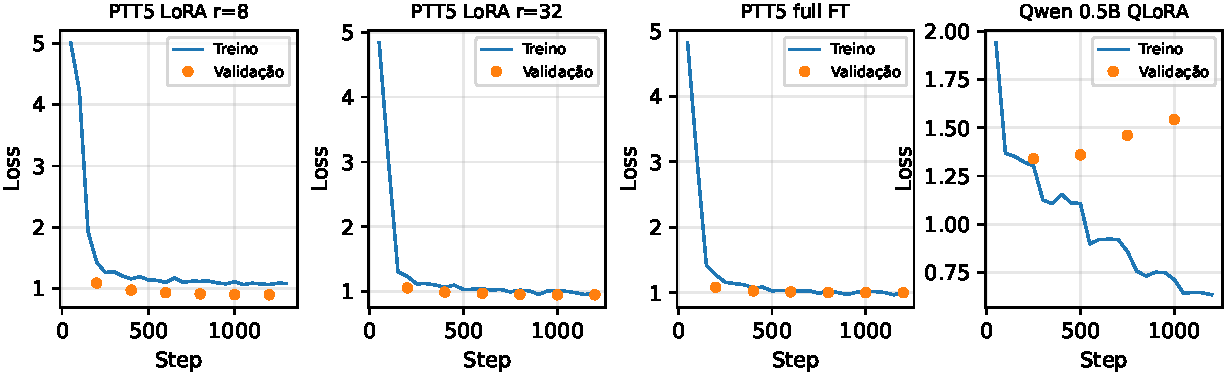
\includegraphics[width=\textwidth]{figs/loss_curves}
\caption{Curvas de perda durante o fine-tuning: (a) PTT5-small
          LoRA rank=8 (eval\_loss 0,996), (b) LoRA rank=32 (0,949),
          (c) fine-tuning completo (1,001) e (d) Qwen 2.5 0.5B com
          QLoRA (0,695).
          Todos os modelos convergem para um plateau na perda de
          validação. Os eixos y diferem entre painéis devido às
          diferentes ordens de grandeza da perda de cada modelo.}
\label{fig:loss}
\end{figure*}

O Qwen 2.5 0.5B apresentou R-1 de 0,60, SARI de 41,8
e F$\Delta = +9,6$. As simplificações são menos similares
lexicalmente, mas os ganhos de legibilidade são substanciais, superando
o PTT5 em F$\Delta$ (+9,6 vs.\ +2,6 a +4,2).

As tr\^es variantes do PTT5-small superam \textbf{todos} os
resultados de prompting em ROUGE e SARI, apesar de terem 10--100$\times$
menos parâmetros que os LLMs avaliados. O Qwen 2.5 0.5B, treinado com
QLoRA, não atinge o mesmo patamar: a escala reduzida
(0,5B parâmetros) limita o aprendizado mesmo com fine-tuning.
Portanto, o fine-tuning em domínio específico pode superar a lacuna
de escala para modelos a partir de 60M parâmetros na tarefa de
simplificação textual.

\subsection{Desempenho do Chain-of-Thought}

A estratégia CoT foi testada em quatro modelos: Qwen 2.5 7B, Llama 4
Scout, GPT-4o mini e GPT-4o. Em todos os casos, o CoT reduz as métricas
de similaridade em comparação com few-shot: Llama 4 Scout
(R-1 = 0,54, SARI = 34,6), GPT-4o mini (R-1 = 0,56, SARI = 34,6),
GPT-4o (R-1 = 0,53, SARI = 34,0) e
Qwen 2.5 7B (R-1 = 0,62, SARI = 37,4). A queda é estatisticamente
significativa para todos os quatro modelos (Llama 4 Scout vs.\
CoT: $p=0,0028$ em R1, $p<0,0001$ em SARI; GPT-4o mini vs.\
CoT: $p<0,0001$ em R1 e SARI; GPT-4o vs.\
CoT: $p<0,0001$ em R1 e SARI; Qwen 2.5 7B vs.\
CoT: $p<0,0001$ em R1 e SARI).

Em legibilidade, o CoT do Llama 4 Scout mantém ganho de
F$\Delta = +13,4$ (vs.\ +13,2 do few-shot, diferença não
significativa, $p=0,87$), o GPT-4o mini CoT obtém
F$\Delta = +12,0$ (vs.\ +10,3 do few-shot, também não
significativo, $p=0,13$), e o GPT-4o CoT obtém
F$\Delta = +11,5$ (vs.\ +9,9 do few-shot, não
significativo, $p=0,19$). O Qwen 2.5 7B CoT, porém, reduz
significativamente o ganho de legibilidade
(F$\Delta = +3,34$ vs.\ +6,21 do few-shot, $p=0,019$),
sugerindo que o impacto do CoT na legibilidade varia conforme o
modelo. Assim, embora o CoT não deteriore a legibilidade na
maioria dos casos, ele reduz consistentemente a similaridade com a
referência, confirmando que o raciocínio passo a passo não
beneficia a simplificação textual na maior parte dos modelos. A
tarefa de simplificação pode não se beneficiar da cadeia de
raciocínio explícita, possivelmente por não exigir inferência
complexa ou raciocínio simbólico.

\subsection{Significância Estatística}

Para verificar se as diferenças observadas entre os modelos são
estatisticamente significativas, realizamos um teste de bootstrap
pareado com 10.000 iterações para cada par de modelos, em cada
métrica. Para controlar o erro tipo I devido às múltiplas
comparações (25 pares $\times$ 6 métricas = 150 testes),
aplicamos a correção de Holm-Bonferroni \citep{holm1979} por
métrica.
A Tabela~\ref{tab:significancia} apresenta as médias
das métricas e grupos de significância (sobrescritos iguais indicam
que não há diferença significativa após a correção,
$\alpha = 0,05$).

\begin{table*}[htbp]
\centering
\caption{Grupos de signific\^ancia (corre\c{c}\~ao de Holm-Bonferroni,
         $\alpha = 0,05$, bootstrap pareado, 10.000 itera\c{c}\~oes).
         Sobrescritos iguais = sem diferen\c{c}a significativa ap\'os
         corre\c{c}\~ao.}
\label{tab:significancia}
\footnotesize
\setlength{\tabcolsep}{3pt}
\begin{tabular}{l c c c c c c}
\toprule
Modelo & R-1 & SARI & F$\Delta$ & Fog$\Delta$ & R1$_{OP}$ & BS$_{OP}$ \\
\midrule
GPT-4o mini          & $0,645^{\text{\tiny a}}$   & $39,2^{\text{\tiny a}}$   & $+10,31^{\text{\tiny a}}$  & $-2,82^{\text{\tiny a}}$  & $0,743^{\text{\tiny a}}$  & $0,904^{\text{\tiny a}}$ \\
GPT-4o               & $0,634^{\text{\tiny a}}$   & $39,2^{\text{\tiny ab}}$  & $+9,89^{\text{\tiny a}}$   & $-2,70^{\text{\tiny a}}$  & $0,721^{\text{\tiny b}}$  & $0,904^{\text{\tiny a}}$ \\
Claude S. 4.6        & $0,662^{\text{\tiny a}}$   & $42,6^{\text{\tiny b}}$   & $+9,97^{\text{\tiny a}}$   & $-3,05^{\text{\tiny a}}$  & $0,756^{\text{\tiny a}}$  & $0,909^{\text{\tiny a}}$ \\
Qwen 2.5 7B          & $0,664^{\text{\tiny a}}$   & $41,7^{\text{\tiny a}}$   & $+6,21^{\text{\tiny b}}$   & $-2,34^{\text{\tiny a}}$  & $0,776^{\text{\tiny c}}$  & $0,905^{\text{\tiny ae}}$ \\
Llama 4 Scout        & $0,576^{\text{\tiny b}}$   & $38,7^{\text{\tiny a}}$   & $+13,23^{\text{\tiny ac}}$ & $-3,95^{\text{\tiny b}}$  & $0,653^{\text{\tiny d}}$  & $0,865^{\text{\tiny b}}$ \\
Llama 4 Scout CoT    & $0,537^{\text{\tiny c}}$   & $34,6^{\text{\tiny c}}$   & $+13,41^{\text{\tiny c}}$  & $-2,96^{\text{\tiny c}}$  & $0,587^{\text{\tiny e}}$  & $0,854^{\text{\tiny bd}}$ \\
GPT-4o mini CoT      & $0,559^{\text{\tiny c}}$   & $34,6^{\text{\tiny cd}}$  & $+12,00^{\text{\tiny ac}}$ & $-2,37^{\text{\tiny ac}}$ & $0,629^{\text{\tiny f}}$  & $0,874^{\text{\tiny c}}$ \\
GPT-4o CoT           & $0,531^{\text{\tiny c}}$   & $34,0^{\text{\tiny c}}$   & $+11,51^{\text{\tiny c}}$  & $-2,73^{\text{\tiny c}}$  & $0,579^{\text{\tiny e}}$  & $0,856^{\text{\tiny d}}$ \\
Qwen 2.5 7B CoT      & $0,616^{\text{\tiny d}}$   & $37,4^{\text{\tiny d}}$   & $+3,34^{\text{\tiny b}}$   & $-1,24^{\text{\tiny d}}$  & $0,730^{\text{\tiny g}}$  & $0,908^{\text{\tiny e}}$ \\
PTT5 LoRA r=8        & $0,743^{\text{\tiny e}}$   & $55,2^{\text{\tiny e}}$   & $+2,58^{\text{\tiny d}}$   & $-0,95^{\text{\tiny e}}$  & $0,933^{\text{\tiny h}}$  & $0,970^{\text{\tiny f}}$ \\
PTT5 LoRA r=32       & $0,729^{\text{\tiny e}}$   & $53,1^{\text{\tiny e}}$   & $+4,17^{\text{\tiny e}}$   & $-1,48^{\text{\tiny f}}$  & $0,910^{\text{\tiny i}}$  & $0,959^{\text{\tiny g}}$ \\
PTT5 full FT         & $0,743^{\text{\tiny e}}$   & $55,5^{\text{\tiny e}}$   & $+3,74^{\text{\tiny e}}$   & $-1,17^{\text{\tiny ef}}$ & $0,927^{\text{\tiny hi}}$ & $0,966^{\text{\tiny fg}}$ \\
Qwen 2.5 0.5B FT     & $0,603^{\text{\tiny a}}$   & $41,8^{\text{\tiny a}}$   & $+9,61^{\text{\tiny a}}$   & $-2,68^{\text{\tiny a}}$  & $0,704^{\text{\tiny a}}$  & $0,890^{\text{\tiny a}}$ \\
\bottomrule
\end{tabular}
\end{table*}

Os resultados de R1 mostram que os modelos few-shot (GPT-4o mini,
GPT-4o, Claude S. 4.6 e Qwen 2.5 7B) e o Qwen 2.5 0.5B FT formam o grupo
superior ($a$); Llama 4 Scout ($b$) é intermediário; Llama 4 Scout CoT,
GPT-4o mini CoT e GPT-4o CoT ($c$) são os piores do prompting;
Qwen 2.5 7B CoT ($d$) é significativamente melhor que os demais CoT,
mas abaixo do few-shot; e os três PTT5 ($e$) lideram isoladamente,
sem diferença entre si.
Em SARI, os PTT5 ($e$) formam o grupo superior, seguidos por
Claude S. 4.6 ($b$); Qwen 2.5 7B CoT ($d$) supera os demais CoT;
Llama 4 Scout CoT e GPT-4o CoT ($c$) ficam abaixo, e GPT-4o mini CoT ($cd$)
é intermediário entre os CoT. O Qwen 2.5 0.5B FT ($a$) é
equivalente aos modelos de prompting nesta métrica.
Em F$\Delta$, os três PTT5 ($d$) produzem os menores ganhos de
legibilidade; Qwen 2.5 7B e Qwen 2.5 7B CoT ($b$) formam grupo
intermediário; Llama 4 Scout ($ac$), Llama 4 Scout CoT ($c$) e
GPT-4o CoT ($c$) lideram com os maiores ganhos.
O Qwen 2.5 0.5B FT ($a$) é equivalente aos modelos proprietários de
prompting (GPT-4o mini, GPT-4o e Claude S. 4.6) em F$\Delta$,
confirmando sua capacidade de simplificação lexical mesmo com 0,5B
parâmetros.

\subsection{Avaliação LLM-as-Judge}

A Tabela~\ref{tab:llmjudge} apresenta os resultados da avaliação do
LLM-judge (200 amostras, 3 execuções). A referência humana
(\textit{sanity check}) obteve 4,86/5,00/4,92, confirmando que o juiz
está bem calibrado.
O desvio padrão entre as três execuções foi inferior a 0,02 em
todas as dimensões, indicando alta reprodutibilidade.

\begin{table*}[htbp]
\centering
\caption{Avaliação LLM-as-judge (Gemini 3.1 Flash Lite) ---
         médias por modelo (Likert 1--5, 3 execuções, 200 amostras).
         Todos os modelos de prompting utilizaram a estratégia
         few-shot.}
\label{tab:llmjudge}
\footnotesize
\setlength{\tabcolsep}{3pt}
\begin{tabular}{l r r r r r r}
\toprule
Modelo & \multicolumn{2}{c}{Simplicidade}
       & \multicolumn{2}{c}{Fluência}
       & \multicolumn{2}{c}{Adequação} \\
       & $M$ & $\sigma$ & $M$ & $\sigma$ & $M$ & $\sigma$ \\
\midrule
Llama 4 Scout         & 4,68 & 0,63 & 4,80 & 0,78 & 4,72 & 0,72 \\
Qwen 2.5 7B           & 4,51 & 0,69 & 4,90 & 0,41 & 4,74 & 0,59 \\
GPT-4o                & 4,73 & 0,54 & 5,00 & 0,00 & 4,90 & 0,31 \\
Claude S. 4.6         & 4,55 & 0,77 & 5,00 & 0,00 & 4,77 & 0,45 \\
GPT-4o mini           & 4,71 & 0,54 & 4,99 & 0,12 & 4,87 & 0,34 \\
PTT5 LoRA r=8         & 2,43 & 1,48 & 4,91 & 0,46 & 4,63 & 0,89 \\
PTT5 LoRA r=32        & 2,73 & 1,56 & 4,84 & 0,68 & 4,50 & 0,99 \\
PTT5 full FT          & 2,55 & 1,53 & 4,86 & 0,65 & 4,57 & 0,96 \\
Qwen 2.5 0.5B FT      & 3,72 & 1,20 & 4,19 & 1,24 & 3,52 & 1,44 \\
\midrule
Ref. Humana (sanity)  & 4,86 & 0,58 & 5,00 & 0,06 & 4,92 & 0,45 \\
\bottomrule
\end{tabular}
\end{table*}

A Tabela~\ref{tab:llmjudge_ranking} apresenta o
ranqueamento completo por dimensão.

\begin{table*}[htbp]
\centering
\caption{Ranking dos modelos por dimensão (LLM-as-judge,
         Likert 1--5, 3 execuções).}
\label{tab:llmjudge_ranking}
\footnotesize
\setlength{\tabcolsep}{3pt}
\begin{tabular}{l c c c}
\toprule
Rank & Simplicidade & Fluência & Adequação \\
\midrule
1 & GPT-4o (4,73)       & GPT-4o (5,00)        & GPT-4o (4,90) \\
2 & GPT-4o mini (4,71)   & Claude S. 4.6 (5,00) & GPT-4o mini (4,87) \\
3 & Llama 4 Scout (4,68) & GPT-4o mini (4,99)   & Claude S. 4.6 (4,77) \\
4 & Claude S. 4.6 (4,55) & PTT5 LoRA r=8 (4,91)      & Qwen 2.5 7B (4,74) \\
5 & Qwen 2.5 7B (4,51)   & Qwen 2.5 7B (4,90)   & Llama 4 Scout (4,72) \\
6 & Qwen 0.5B FT (3,72)  & PTT5 full FT (4,86)  & PTT5 LoRA r=8 (4,63) \\
7 & PTT5 LoRA r=32 (2,73)     & PTT5 LoRA r=32 (4,84)     & PTT5 full FT (4,57) \\
8 & PTT5 full FT (2,55)  & Llama 4 Scout (4,80) & PTT5 LoRA r=32 (4,50) \\
9 & PTT5 LoRA r=8 (2,43)      & Qwen 0.5B FT (4,19)  & Qwen 0.5B FT (3,52) \\
\bottomrule
\end{tabular}
\end{table*}

Os modelos de prompting obtêm notas altas em simplicidade
(4,51--4,73), fluência (4,80--5,00) e adequação (4,72--4,90).
O GPT-4o lidera em simplicidade (4,73) e adequação (4,90);
Claude e GPT-4o atingem fluência máxima (5,00).
O Qwen 2.5 7B tem simplicidade ligeiramente inferior
(4,51), o que é coerente com seu ganho de legibilidade mais modesto.
O Llama 4 Scout, apesar de liderar em F$\Delta$, tem a fluência
mais baixa entre os modelos de prompting (4,80) por causa de
ocasionais quebras de estruturas gramaticais.

Os modelos fine-tunados revelam padrões qualitativos importantes.
As três variantes do PTT5 obtêm as menores notas de simplicidade
(2,43 a 2,73), confirmando que o PTT5 tende a copiar o texto original
com ajustes mínimos independentemente da configuração de treino.
Suas fluências (4,84--4,91) e adequações (4,50--4,63) são comparáveis
aos modelos de prompting, indicando que as saídas são gramaticais
e semanticamente válidas, mas sem simplificar efetivamente.
O PTT5 LoRA r=32 apresenta a melhor simplicidade entre as três
variantes (2,73), coerente com seu maior F$\Delta$ (+4,2).
O Qwen 2.5 0.5B FT, por sua vez, atinge a maior simplicidade entre
os fine-tunados (3,72), refletindo seu maior ganho de legibilidade,
mas apresenta a menor adequação (3,52) e fluência (4,19) entre todos
os modelos, consistentes com as alucinações semânticas observadas
(ex. inversão de sentido em ``legislação branda'' $\to$ ``lei muito
rigorosa'').

A correlação de Spearman entre as notas do LLM-judge e o ROUGE-1
revela relações complementares. Simplicidade correlaciona-se
negativamente com ROUGE-1 ($\rho = -0,113$, $p < 0,001$):
modelos que maximizam similaridade lexical
(como o PTT5) tendem a produzir simplificações percebidas como
menos simplificadas pelo juiz, embora o efeito seja pequeno
(R$^2 < 0,02$). Fluência ($\rho = 0,130$) e adequação ($\rho = 0,246$)
apresentam correlações positivas fracas com ROUGE-1 ($p < 0,001$):
maior similaridade lexical está associada a saídas
mais fluentes e adequadas, mas o efeito é pequeno.
Em conjunto, as métricas automáticas e o LLM-judge capturam aspectos
complementares da simplificação textual.

\subsection{Análise de Concordância entre Juízes Automáticos}

Para avaliar a robustez da avaliação LLM-as-judge, repetimos o
experimento com o GPT-4o mini como segundo juiz. A
Tabela~\ref{tab:llmjudge2} apresenta as médias obtidas por cada modelo,
e a Tabela~\ref{tab:agreement} reporta a concordância entre os dois
juízes medida pelo Krippendorff's $\alpha$.

\begin{table*}[htbp]
\centering
\caption{Avaliação LLM-as-judge com GPT-4o mini ---
         médias por modelo (Likert 1--5, 3 execuções, 200 amostras).}
\label{tab:llmjudge2}
\footnotesize
\setlength{\tabcolsep}{3pt}
\begin{tabular}{l r r r}
\toprule
Modelo & Simplicidade & Fluência & Adequação \\
\midrule
Llama 4 Scout        & 3,93 & 4,45 & 4,10 \\
Qwen 2.5 7B          & 3,75 & 4,37 & 4,23 \\
GPT-4o               & 3,94 & 4,46 & 4,20 \\
Claude S. 4.6        & 3,85 & 4,50 & 4,30 \\
GPT-4o mini          & 3,91 & 4,47 & 4,26 \\
PTT5 LoRA r=8        & 2,79 & 4,24 & 4,70 \\
PTT5 LoRA r=32       & 2,90 & 4,20 & 4,59 \\
PTT5 full FT         & 2,83 & 4,21 & 4,66 \\
Qwen 2.5 0.5B FT     & 3,18 & 4,04 & 3,65 \\
\midrule
Ref. Humana (sanity) & 5,00 & 5,00 & 5,00 \\
\bottomrule
\end{tabular}
\end{table*}

O GPT-4o mini como juiz atribui notas sistematicamente mais baixas que
o Gemini: a média geral em simplicidade cai de 4,64 (Gemini) para 3,79
(GPT-4o mini), em fluência de 4,91 para 4,27, e em adequação de 4,77
para 4,23. As
variantes do PTT5, que o Gemini avaliou com simplicidade entre 2,43 e
2,73, recebem notas ligeiramente superiores do GPT-4o mini
(2,79--2,90). O sanity check (referência humana avaliada contra si
mesma) atinge 5,00 em todas as dimensões para ambos os juízes,
confirmando que ambos identificam corretamente o texto de referência.

\begin{table*}[htbp]
\centering
\caption{Concordância entre juízes (Gemini vs.\ GPT-4o mini).
         $\alpha$-Simp/$\alpha$-Flu/$\alpha$-Adeq: Krippendorff's $\alpha$
         inter-juiz por dimensão; $\kappa$: Cohen's $\kappa$ não-ponderado
         (média 3 dims); $\kappa_w$: Cohen's $\kappa_w$ linear
         (média 3 dims); $\alpha_{i}$-G: consistência interna do Gemini
         entre as 3 execuções; $\alpha_{i}$-M: consistência interna do
         GPT-4o mini entre as 3 execuções.}
\label{tab:agreement}
\footnotesize
\setlength{\tabcolsep}{3pt}
\begin{tabular}{l r r r r r r r}
\toprule
Modelo & \multicolumn{1}{c}{$\alpha$-Simp}
       & \multicolumn{1}{c}{$\alpha$-Flu}
       & \multicolumn{1}{c}{$\alpha$-Adeq}
       & \multicolumn{1}{c}{$\kappa$}
       & \multicolumn{1}{c}{$\kappa_w$}
       & \multicolumn{1}{c}{$\alpha_{i}$-G}
       & \multicolumn{1}{c}{$\alpha_{i}$-M} \\
\midrule
GPT-4o mini          &  0,018 & $-0,298$ & $-0,181$ &  0,020  & $-0,013$ & 0,950  & 0,843  \\
GPT-4o               & $-0,012$ & $-0,341$ & $-0,330$ &  0,007  &  0,323  & 0,953  & 0,835  \\
Claude S. 4.6        &  0,288 & $-0,305$ &  0,099  &  0,038  &  0,310  & 0,968  & 0,849  \\
Llama 4 Scout        &  0,039 &  0,352  &  0,199  &  0,055  & $-0,031$ & 0,959  & 0,832  \\
Qwen 2.5 7B          &  0,145 & $-0,120$ &  0,248  &  0,073  & $-0,029$ & 0,959  & 0,845  \\
PTT5 LoRA r=8        &  0,579 & $-0,155$ &  0,734  &  0,240  & $-0,092$ & 0,949  & 0,874  \\
PTT5 LoRA r=32       &  0,615 &  0,128  &  0,765  &  0,252  & $-0,115$ & 0,969  & 0,890  \\
PTT5 full FT         &  0,647 &  0,069  &  0,780  &  0,239  & $-0,109$ & 0,977  & 0,879  \\
Qwen 2.5 0.5B FT     &  0,360 &  0,398  &  0,759  &  0,222  & $-0,138$ & 0,977  & 0,898  \\
\midrule
Média                &  0,265 & $-0,027$ &  0,306  &  0,115  &  0,110  & 0,962  & 0,861  \\
\bottomrule
\end{tabular}
\end{table*}

Os resultados revelam um padrão claro: a concordância entre juízes
varia substancialmente conforme o tipo de modelo e a dimensão avaliada.
Para modelos fine-tunados (PTT5 e Qwen 0.5B), a concordância em
simplicidade e adequação é de moderada a substancial
($\alpha = 0,360$ a $0,780$), indicando que os juízes convergem ao
avaliar as diferenças mais marcantes entre cópias próximas do original
(PTT5) e textos simplificados. Para modelos de prompting (LLMs),
no entanto, a concordância é baixa ou negativa em todas as dimensões
($\alpha = -0,341$ a $0,352$), sugerindo que, quando as diferenças
entre as saídas são mais sutis, cada juiz aplica critérios distintos.

A fluência apresenta a pior concordância média ($\alpha = -0,027$),
com valores negativos para a maioria dos modelos. Isso indica que
os dois juízes discordam sistematicamente sobre o que constitui um
texto ``natural e bem formado'' em português, possivelmente porque o
Gemini é mais tolerante a pequenas variações estruturais enquanto o
GPT-4o mini penaliza desvios da norma padrão. A adequação é a dimensão
com melhor concordância ($\alpha = 0,306$), especialmente para modelos
fine-tunados ($\alpha \geq 0,75$), sugerindo que a preservação de
significado é o critério mais objetivo entre os dois juízes.

O Cohen's $\kappa$ (não-ponderado) fornece uma visão complementar:
para concordância exata, os valores são baixos ($\kappa = 0,115$ em
média), mesmo para os modelos fine-tunados ($\kappa \approx 0,24$),
refletindo que os juízes raramente atribuem a mesma nota numérica
exata. O $\kappa_w$ (ponderado linear), que considera discordâncias
parciais, mostra concordância ligeiramente superior para alguns
modelos de prompting (GPT-4o: $\kappa_w = 0,323$; Claude:
$\kappa_w = 0,308$) -- nestes casos, ambos os juízes atribuíram notas
máximas (5,0) em fluência para todas as amostras, resultando em
concordância perfeita nessa dimensão. Para os demais modelos,
$\kappa_w$ é consistentemente negativo, um artefato conhecido do
$\kappa_w$ quando as distribuições marginais dos dois juízes diferem
sistematicamente \citep{feinstein1990kappa}.

A consistência interna de cada juiz (Krippendorff's $\alpha$ entre as
3 execuções) é elevada para ambos os modelos: Gemini apresentou
$\alpha_i = 0,962$ em média e GPT-4o mini $\alpha_i = 0,861$,
superiores ao limiar de 0,80 para concordância quase perfeita. Isto
confirma que 3 execuções com temperatura 0,3 são suficientes para
estabilizar as avaliações de cada juiz individualmente, e que a baixa
concordância entre os juízes reflete divergências reais de critério,
não ruído amostral. Nota-se também que o Gemini é ligeiramente mais
consistente que o GPT-4o mini ($\alpha_i$ médio 0,962 vs.\ 0,861),
especialmente para modelos de prompting ($\Delta \approx 0,12$), onde
as diferenças entre as saídas são mais sutis e a variabilidade das
avaliações do GPT-4o mini é maior.

Esse resultado afeta a metodologia
LLM-as-judge: a escolha do modelo juiz impacta as
avaliações, especialmente quando as diferenças entre os sistemas
avaliados são pequenas. Recomenda-se o uso de múltiplos juízes
automáticos e a reportação da concordância entre eles como parte da
avaliação.

\section{Discussão}

\subsection{Tradeoff Similaridade versus Legibilidade}

Os resultados revelam um tradeoff entre similaridade com a referência
e ganho de legibilidade. O few-shot frequentemente maximiza ambas, mas
o grau do tradeoff varia entre modelos: no Llama 4 Scout, o ganho de
legibilidade é máximo independentemente da estratégia; no Qwen 2.5 7B,
o few-shot atinge a maior similaridade mas com ganho de legibilidade
significativamente menor, sugerindo que o tradeoff é dependente do
modelo.

A avaliação LLM-as-judge corrobora este tradeoff: as três variantes
do PTT5, que maximizam similaridade com a referência, obtêm as piores
notas de simplicidade do LLM-judge, enquanto o Llama 4 Scout, que
lidera em ganho de legibilidade, mantém simplicidade alta. Isto sugere
que as métricas automáticas de similaridade (ROUGE, SARI) e o
LLM-judge capturam aspectos complementares: ROUGE mede sobreposição
lexical, enquanto o juiz avalia o efeito perceptual da simplificação.

Um resultado relevante é que quatro modelos superam o
baseline humano de legibilidade (Llama 4 Scout, Claude S. 4.6,
GPT-4o mini e GPT-4o zero-shot), indicando que LLMs podem simplificar
além do nível das referências do dataset. Isto sugere que as
referências do PorSimplesSent, embora válidas, não representam o
``nível máximo'' de simplificação possível: as referências humanas
priorizam a preservação do significado sobre a maximalidade da
simplificação, e ganhos de legibilidade além delas não implicam
necessariamente simplificações superiores. As notas de adequação do
LLM-judge (e.g., Llama 4 Scout com adequação 4,72) indicam que o
ganho não compromete o significado na maioria dos casos, mas as
limitações dessa avaliação (Seção~5.5) devem ser consideradas.
A escolha da estratégia
ideal depende do objetivo da aplicação: para sistemas que devem seguir
um padrão pré-definido, o few-shot é preferível; para equilibrar
similaridade e acessibilidade, a escolha do modelo é tão importante
quanto a estratégia de prompting.

\subsection{Custo-Benefício dos Modelos}

O Qwen 2.5 7B destaca-se como a alternativa de melhor custo-benefício.
Seu desempenho em similaridade empata com o Claude S. 4.6, e seu
R1$_{OP}$ elevado indica simplificações conservadoras e próximas ao
estilo humano. Além disso, seu custo por token via OpenRouter é menor
que o do GPT-4o mini, e o modelo pode ser executado localmente para
eliminar custos de acesso via API. O GPT-4o (full), apesar de ser o
modelo de maior porte, não apresentou vantagens sobre o mini na tarefa
de simplificação, sugerindo que o fine-tuning da versão mini para
instruções específicas pode ser mais benéfico que o aumento de escala.
O Claude Sonnet 4.6 apresenta desempenho comparável, empatando em R1
com o Qwen e superando-o em SARI, com custo de API idêntico.
O LLM-judge confirma a equivalência entre ambos. O Llama 4 Scout,
apesar do menor desempenho em similaridade, oferece o maior contexto
(10M tokens) e os maiores ganhos de legibilidade, sendo útil para
aplicações que priorizam simplificação mais agressiva.

Para uma comparação de custo unificada, modelos de prompting via API
incorrem em custo por chamada, enquanto o fine-tuning requer
investimento inicial em treinamento (GPU local ou em nuvem) mas
torna a inferência posterior essencialmente gratuita. Para aplicações
com alto volume de simplificações, o fine-tuning torna-se mais
econômico; para usos esporádicos, o prompting via API é mais prático.

\subsection{Fine-Tuning versus Prompting}

O fine-tuning do PTT5-small (60M) superou todos os resultados de
prompting em métricas de similaridade, mas isso não significa que seja
sempre superior: gerou simplificações excessivamente conservadoras
(R1$_{OP} \approx 0,93$, F$\Delta = +2,6$ a $+4,2$), praticamente
copiando o original com pequenos ajustes. O LLM-judge corrobora esta
análise: as três variantes do PTT5 obtêm as menores notas de
simplicidade entre todos os modelos, enquanto fluência e adequação
são comparáveis aos de prompting.

Uma análise das curvas de perda (Figura~\ref{fig:loss}) descarta a
hipótese de underfitting: todas as variantes convergiram para um
plateau, sugerindo que uma possível explicação para o comportamento
conservador é uma característica inerente ao modelo, que por ter
sido pré-treinado para reconstruir o texto original, tende a
copiá-lo. O Qwen 2.5 0.5B, com arquitetura decoder-only, atinge
maior ganho de legibilidade (F$\Delta = +9,6$) mas sofre de alucinações
semânticas (adequação 3,52), refletindo sua escala reduzida.

A principal vantagem do prompting é a flexibilidade: um mesmo modelo
pode ser adaptado a diferentes estilos de simplificação apenas
alterando o prompt. O fine-tuning oferece desempenho superior em
similaridade quando há dados rotulados, mas o comportamento
conservador do PTT5-small contrasta com o Qwen 2.5 0.5B, refletindo
diferenças arquiteturais: o encoder-decoder T5 é treinado para
span corruption, enquanto o decoder-only Qwen é treinado para predizer
o próximo token, o que pode favorecer maior diversidade lexical nas
saídas. Exemplos representativos são apresentados no
Apêndice~\ref{apendice:qualitativa}.

\subsection{Robustez ao N\'umero de Exemplos Few-Shot}

A estrat\'egia few-shot foi avaliada com k=3 exemplos, valor comumente
adotado na literatura de simplifica\c{c}\~ao textual \citep{brown2020}.
Para verificar a sensibilidade dos resultados ao n\'umero de exemplos,
realizamos uma an\'alise de robustez com k = 1, 3, 5 e 7 no GPT-4o mini
(Tabela~\ref{tab:ablation}).
Os resultados mostram que as m\'etricas de similaridade melhoram
com mais exemplos: SARI sobe de 39,3 (k=1) para 42,2 (k=7),
e R1 de 0,652 para 0,675.
O ganho de legibilidade (F$\Delta$) varia entre +8,3 (k=7) e +10,7 (k=3),
sem tendência clara.
As diferen\c{c}as s\~ao moderadas: a varia\c{c}\~ao m\'axima \'e de
aproximadamente 8\% em SARI e 4\% em R1, e n\~ao alteram o
posicionamento relativo do GPT-4o mini em rela\c{c}\~ao aos demais
modelos. Assim, k=3 representa um equil\'ibrio razo\'avel entre
custo computacional e qualidade das simplifica\c{c}\~oes.

\begin{table*}[htbp]
\centering
\caption{An\'alise de robustez ao n\'umero de exemplos few-shot (k)
no GPT-4o mini.}
\label{tab:ablation}
\footnotesize
\begin{tabular}{c c c c c c}
\toprule
k & R1 & SARI & F$\Delta$ & Fog$\Delta$ & R1$_{OP}$ \\
\midrule
1 & 0,652 & 39,3 & +9,1 & $-2,2$ & 0,751 \\
3 & 0,65 & 39,2 & +10,7 & $-2,9$ & 0,743 \\
5 & 0,676 & 41,4 & +8,4 & $-2,2$ & 0,791 \\
7 & 0,675 & 42,2 & +8,3 & $-2,3$ & 0,793 \\
\bottomrule
\end{tabular}
\end{table*}

\subsection{Limitações}

Este trabalho apresenta limitações que devem ser consideradas. O
dataset utilizado
(PorSimplesSent) contém apenas pares ORI--NAT de um domínio
jornalístico, não abrangendo outros gêneros textuais. Modelos de
raciocínio (como DeepSeek e Nemotron) não puderam ser completamente
avaliados devido ao elevado consumo de tokens decorrente do raciocínio
interno.

A contagem de sílabas para o português foi feita com um algoritmo
heurístico que, embora suficiente para análise comparativa, pode conter
imprecisões em palavras com hiatos ou ditongos complexos.

A avaliação LLM-as-judge, embora útil como complemento às
métricas automáticas, apresenta limitações próprias. Os
modelos juízes (Gemini 3.1 Flash Lite e GPT-4o mini) podem ter vieses
inerentes, incluindo preferência por textos mais longos ou por padrões
linguísticos específicos. A baixa concordância entre os dois juízes
($\alpha = 0,181$ em média, chegando a $\alpha < 0$ em fluência)
indica que a avaliação LLM-as-judge é altamente dependente do modelo
juiz escolhido, especialmente para modelos de prompting onde as
diferenças entre as saídas são mais sutis. A avaliação com
juízes automáticos não captura a diversidade de perspectivas que
múltiplos avaliadores humanos proporcionariam.

O fine-tuning completo do PTT5-small convergiu para perda de validação
de 1,001, comparável aos adaptadores LoRA (0,95--1,00), indicando
que os dados disponíveis (1.953 pares) são suficientes para treinar
60 milhões de parâmetros, mas o comportamento conservador persiste.
Experimentos com mais dados ou técnicas de regularização adicionais
poderiam alterar este resultado. Cada configuração de fine-tuning foi
treinada uma única vez (sem variação de semente aleatória), o que
limita a robustez das comparações entre variantes.

\section{Conclusão}

Este trabalho comparou cinco LLMs e
quatro modelos fine-tunados para simplificação textual em português
brasileiro. LLMs de grande porte realizam simplificação sem fine-tuning
com desempenho satisfatório: few-shot (k=3) produz os melhores
resultados de similaridade e legibilidade, enquanto CoT reduz
consistentemente a similaridade sem benefícios de legibilidade.
O fine-tuning do PTT5-small (60M) supera todos os resultados de
prompting com modelos muito maiores (7B--17B) em similaridade
(ROUGE-1 até 0,74, SARI até 55,5), mas com comportamento conservador
(F$\Delta \leq +4,2$). Métricas de similaridade e legibilidade devem
ser reportadas conjuntamente para uma avaliação completa.
A avaliação LLM-as-judge revela baixa concordância entre juízes
($\alpha = 0,181$), indicando sensibilidade à escolha do modelo juiz
e limitando a confiabilidade da avaliação automática isolada.

Trabalhos futuros incluem: (i) expandir a avaliação para todo o
dataset de 2.370 pares, verificando se os padrões observados se
mantêm com maior cobertura de amostras e permitindo análises por
estrato de tamanho e complexidade sintática; (ii) realizar
fine-tuning do Qwen 2.5 7B com LoRA para investigar se uma base
maior (7B parâmetros) combinada com treinamento supervisionado
atinge similaridade próxima ao PTT5 com ganhos de legibilidade
superiores; (iii) realizar avaliação com
juízes humanos para calibrar as métricas automáticas e o LLM-judge;
(iv) investigar se prompts estilísticos (com nível-alvo de
simplificação explícito) podem reduzir a lacuna entre similaridade e
legibilidade em modelos fine-tunados.

\section*{Disponibilidade de Código e Dados}

O código-fonte utilizado neste trabalho está disponível sob licença
GPLv3 em \url{https://github.com/jsansao/llm-text-simplification-ptbr}.
O dataset PorSimplesSent~\citep{caseli2009} é distribuído sob
licença CC BY 4.0
(\url{https://github.com/sidleal/porsimplessent}).
A amostra estratificada de 200 pares, as predições completas de
todos os modelos e as adaptações dos índices de legibilidade para o
português acompanham o repositório.

\section*{Agradecimentos}
Os autores agradecem à Universidade Federal de São João del-Rei (UFSJ)
pelo apoio institucional.

\bibliography{artigo}

\appendix
\section{Análise Qualitativa}
\label{apendice:qualitativa}

Esta seção apresenta as predições dos modelos em cinco amostras
selecionadas da amostra estratificada de 200 pares: a de maior consenso
(\#158, R1 médio 0,964), a de maior dificuldade (\#16, R1 médio 0,019),
duas de maior divergência (\#103, std=0,296; \#127, std=0,284) e a de
maior comprimento (\#141, 52 tokens).

\subsection{Exemplos Selecionados}

\footnotesize

\medskip
\paragraph*{Amostra \#158 (consenso, R1 médio=0,964).}

\textbf{Original:} A identificação e descrição está sendo feita com a ajuda de Marina Capelari, do Instituto de Botânica de São Paulo, e Dennis Desjardin, da Universidade Estadual de San Francisco (Unidos).

\textbf{Referência:} A identificação e descrição está sendo feita com a ajuda de Marina Capelari, do Instituto de Botânica de São Paulo, e Dennis Desjardin, da Universidade Estadual de San Francisco, Unidos.

\textbf{GPT-4o mini:} A identificação e descrição estão sendo feitas com a ajuda de Marina Capelari, do Instituto de Botânica de São Paulo, e Dennis Desjardin, da Universidade Estadual de San Francisco.

\textbf{GPT-4o:} A identificação e descrição está sendo feita com a ajuda de Marina Capelari, do Instituto de Botânica de São Paulo, e Dennis Desjardin, da Universidade Estadual de San Francisco.

\textbf{Claude S. 4.6:} A identificação e descrição está sendo feita com a ajuda de Marina Capelari, do Instituto de Botânica de São Paulo, e Dennis Desjardin, da Universidade Estadual de San Francisco.

\textbf{Llama 4 Scout:} A identificação e descrição estão sendo feitas com a ajuda de Marina Capelari, do Instituto de Botânica de São Paulo, e Dennis Desjardin, da Universidade Estadual de San Francisco.

\textbf{Qwen 2.5 7B:} A identificação e descrição foram feitas com a ajuda de Marina Capelari, do Instituto de Botânica de São Paulo, e Dennis Desjardin, da Universidade Estadual de San Francisco.

\textbf{PTT5 LoRA r=8:} A identificação e descrição está sendo feita com a ajuda de Marina Capelari, do Instituto de Botânica de São Paulo, e Dennis Desjardin, da Universidade Estadual de San Francisco.

\textbf{PTT5 LoRA r=32:} A identificação e descrição está sendo feita com a ajuda de Marina Capelari, do Instituto de Botânica de São Paulo, e Dennis Desjardin, da Universidade Estadual de San Francisco.

\textbf{PTT5 full FT:} A identificação e descrição está sendo feita com a ajuda de Marina Capelari, do Instituto de Botânica de São Paulo, e Dennis Desjardin, da Universidade Estadual de San Francisco (Unidos).

\textbf{Qwen 2.5 0.5B FT:} A identificação e descrição estão sendo feitas com a ajuda de Marina Capelari, do Instituto de Botânica de São Paulo, e Dennis Desjardin, da Universidade Estadual de San Francisco.

\bigskip
\paragraph*{Amostra \#16 (difícil, R1 médio=0,019).}

\textbf{Original:} Sem contra-indicações, as gotinhas devem ser tomadas até mesmo por crianças com febre.

\textbf{Referência:} Maria Aparecida müller vilarino é coordenadora do núcleo de vacinação da Secretaria Municipal da Saúde.

\textbf{GPT-4o mini:} As gotinhas podem ser tomadas por crianças com febre.

\textbf{GPT-4o:} As gotinhas podem ser tomadas até por crianças com febre.

\textbf{Claude S. 4.6:} As gotinhas devem ser tomadas até mesmo por crianças com febre.

\textbf{Llama 4 Scout:} As gotinhas podem ser dadas para crianças com febre, sem problemas.

\textbf{Qwen 2.5 7B:} As gotinhas podem ser tomadas até mesmo por crianças com febre, pois não causam problemas.

\textbf{PTT5 LoRA r=8:} Sem contra-indicações, as gotinhas devem ser tomadas até mesmo por crianças com febre.

\textbf{PTT5 LoRA r=32:} Sem contra-indicações, as gotinhas devem ser tomadas até mesmo por crianças com febre.

\textbf{PTT5 full FT:} Sem contra-indicações, as gotinhas devem ser tomadas até mesmo por crianças com febre.

\textbf{Qwen 2.5 0.5B FT:} Simplifique o texto a seguir: Sem contraindicoções, as gotinhas devem ser tomadas até mesmo por crianças com febre.

\bigskip
\paragraph*{Amostra \#103 (divergência, std=0,296).}

\textbf{Original:} -- O fórum retrata a diversidade da comunidade de software livre, onde todos os grupos, projetos e iniciativas têm espaço.

\textbf{Referência:} -- O fórum reproduz a variedade da comunidade de software livre, onde todos os grupos, projetos e iniciativas têm espaço.

\textbf{GPT-4o mini:} O fórum mostra a diversidade da comunidade de software livre, onde todos os grupos e projetos têm espaço.

\textbf{GPT-4o:} -- O fórum mostra a diversidade da comunidade de software livre, onde todos têm espaço.

\textbf{Claude S. 4.6:} -- O fórum mostra a diversidade da comunidade de software livre, onde todos os grupos e projetos têm espaço.

\textbf{Llama 4 Scout:} O f

\textbf{Qwen 2.5 7B:} O fórum mostra a diversidade da comunidade de software livre, onde todos os grupos, projetos e iniciativas têm espaço.

\textbf{PTT5 LoRA r=8:} -- O fórum retrata a diversidade da comunidade de software livre, onde todos os grupos, projetos e iniciativas têm espaço.

\textbf{PTT5 LoRA r=32:} -- O fórum retrata a diversidade da comunidade de software livre, onde todos os grupos, projetos e iniciativas têm espaço.

\textbf{PTT5 full FT:} -- O fórum retrata a diversidade da comunidade de software livre, onde todos os grupos, projetos e iniciativas têm espaço.

\textbf{Qwen 2.5 0.5B FT:} -- O fórum é um lugar para todas as pessoas que desejam desenvolver software livre.

\bigskip
\paragraph*{Amostra \#127 (divergência: 2\textordfeminine{} maior std, std=0,284).}

\textbf{Original:} O aumento da população de rua, de um lado, é acompanhado da redução dos espaços públicos historicamente usados por mendigos.

\textbf{Referência:} O aumento da população de rua é acompanhado da redução dos espaços públicos historicamente usados por mendigos.

\textbf{GPT-4o mini:} Aumenta a população de rua e diminui os espaços públicos usados por mendigos.

\textbf{GPT-4o:} O número de moradores de rua aumenta, enquanto os espaços públicos usados por mendigos diminuem.

\textbf{Claude S. 4.6:} O número de pessoas em situação de rua cresce, mas os espaços públicos que elas usavam diminuem.

\textbf{Llama 4 Scout:} O aumento do número de pessoas na rua acontece ao mesmo tempo em que diminuem os espaços públicos onde elas costumam ficar.

\textbf{Qwen 2.5 7B:} A simplificação da frase seria: A população de rua está aumentando, enquanto os espaços públicos usados por mendigos estão diminuindo.

\textbf{PTT5 LoRA r=8:} O aumento da população de rua é acompanhado da redução dos espaços públicos historicamente usados por mendigos.

\textbf{PTT5 LoRA r=32:} O aumento da população de rua é acompanhado da redução dos espaços públicos historicamente usados por mendigos.

\textbf{PTT5 full FT:} O aumento da população de rua é acompanhado da redução dos espaços públicos historicamente usados por mendigos.

\textbf{Qwen 2.5 0.5B FT:} Aumenta-se o número de pessoas que vivem em ruas e diminui-se os espaços públicos históricos para mendigos.

\bigskip
\paragraph*{Amostra \#141 (mais longa, 52 tokens).}

\textbf{Original:} Para isso, investe no talento e no desenvolvimento de seus colaboradores, que têm suas atividades pautadas pelo Guia de Ética, Qualidade e Responsabilidade Social, um conjunto de orientações éticas e editoriais destinado a facilitar aos profissionais da RBS o conhecimento dos valores da empresa e sua aplicação prática em situações de trabalho.

\textbf{Referência:} O Guia de Ética é um conjunto de orientações éticas e editoriais destinado a facilitar o conhecimento dos valores da empresa e sua aplicação prática em situações de trabalho.

\textbf{GPT-4o mini:} Ele investe no talento e no desenvolvimento de seus colaboradores. As atividades deles seguem o Guia de Ética, Qualidade e Responsabilidade Social. Esse guia ajuda os profissionais da RBS a entender os valores da empresa e como aplicá-los no trabalho.

\textbf{GPT-4o:} Investe no talento e no desenvolvimento dos colaboradores, seguindo o Guia de Ética, Qualidade e Responsabilidade Social, que orienta os profissionais da RBS sobre os valores da empresa e como aplicá-los no trabalho.

\textbf{Claude S. 4.6:} Para isso, investe no talento e no desenvolvimento de seus colaboradores, que têm suas atividades pautadas pelo Guia de Ética, Qualidade e Responsabilidade Social, um conjunto de orientações éticas e editoriais para ajudar os profissionais da RBS a conhecer os valores da empresa e aplicá-los no trabalho.

\textbf{Llama 4 Scout:} Para isso, a empresa investe no talento e no desenvolvimento de seus colaboradores. Eles seguem um guia de ética, qualidade e responsabilidade social. Esse guia ajuda os profissionais a entender e aplicar os valores da empresa no dia a dia.

\textbf{Qwen 2.5 7B:} Para isso, investe no talento e no desenvolvimento dos colaboradores. As atividades deles seguem o Guia de Ética, Qualidade e Responsabilidade Social. Este guia ajuda os profissionais a entenderem os valores da empresa e a aplicá-los no trabalho.

\textbf{PTT5 LoRA r=8:} Para isso, investe no talento e no desenvolvimento de seus colaboradores, que têm suas atividades pautadas pelo Guia de Ética, Qualidade e Responsabilidade Social.

\textbf{PTT5 LoRA r=32:} Para isso, investe no talento e no desenvolvimento de seus colaboradores, que têm suas atividades pautadas pelo Guia de Ética, Qualidade e Responsabilidade Social.

\textbf{PTT5 full FT:} Para isso, investe no talento e no desenvolvimento de seus colaboradores.

\textbf{Qwen 2.5 0.5B FT:} Aqui está o texto simplificado: \% falha: produziu apenas metatexto sem a simplificação

\end{document}